% !TeX encoding = UTF-8

% 载入 SJTUThesis 模版
\documentclass[type=bachelor, openany, zihao=5]{sjtuthesis}
% 选项
%   type=[doctor|master|bachelor],     % 可选(默认:master),论文类型
%   zihao=[-4|5],                      % 可选(默认:-4),正文字号大小
%   lang=[zh|en|de|ja],                % 可选(默认:zh),论文的主要语言
%   review,                            % 可选(默认:关闭),盲审模式
%   [twoside|oneside],                 % 可选(默认:twoside),双页或单页边距模式
%   [openright|openany],               % 可选(默认:openright),奇数页或任意页开始新章
%   math-style=[ISO|TeX],              % 可选 (默认:ISO),数学符号样式

% 论文基本配置,加载宏包等全局配置
% !TEX root = ./main.tex

\sjtusetup{
  %
  %******************************
  % 注意:
  %   1. 配置里面不要出现空行
  %   2. 不需要的配置信息可以删除
  %******************************
  %
  % 信息录入
  %
  info = {%
    %
    % 标题
    %
    zh / title           = {联邦学习中的高效差分隐私计算},
    en / title           = {A Sample Document for \LaTeX-based SJTU Thesis Template},
    %
    % 标题页标题
    %   可使用“\\”命令手动控制换行
    %
    % zh / display-title   = {上海交通大学学位论文\\ \LaTeX{} 模板示例文档},
    % en / display-title   = {A Sample Document \\ for \LaTeX-based SJTU Thesis Template},
    %
    % 关键词
    %
    zh / keywords        = {上海交大, 饮水思源, 爱国荣校},
    en / keywords        = {SJTU, master thesis, XeTeX/LaTeX template},
    %
    % 姓名
    %
    zh / author          = {叶航宇},
    en / author          = {Mo Mo},
    %
    % 指导教师
    %
    zh / supervisor      = {某某教授},
    en / supervisor      = {Prof. Mou Mou},
    %
    % 副指导教师
    %
    % assoc-supervisor  = {某某教授},
    % assoc-supervisor* = {Prof. Uom Uom},
    %
    % 学号
    %
    id              = {519021911239},
    %
    % 学位
    %   本科生不需要填写
    %
    zh / degree          = {工学硕士},
    en / degree          = {Master of Engineering},
    %
    % 专业
    %
    zh / major           = {计算机科学与技术},
    en / major           = {A Very Important Major},
    %
    % 所属院系
    %
    zh / department      = {电子信息与电气工程学院},
    en / department      = {Depart of XXX},
    %
    % 答辩日期
    %   使用 ISO 格式 (yyyy-mm-dd);默认为当前时间
    %
    % date            = {2014-12-17},
    %
    % 资助基金
    %
    % zh / fund  = {
    %                {国家 973 项目 (No. 2025CB000000)},
    %                {国家自然科学基金 (No. 81120250000)},
    %              },
    % en / fund  = {
    %                {National Basic Research Program of China (Grant No. 2025CB000000)},
    %                {National Natural Science Foundation of China (Grant No. 81120250000)},
    %              },
  },
  %
  % 风格设置
  %
  style = {%
    %
    % 论文标题页 logo 颜色 (red/blue/black)
    %
    % title-logo-color = black,
  },
  %
  % 名称设置
  %
  name = {
    % bib             = {References},
    % ack             = {谢\hspace{\ccwd}辞},
    % achv            = {攻读学位期间完成的论文},
  },
}

% 使用 BibLaTeX 处理参考文献
%   biblatex-gb7714-2015 常用选项
%     gbnamefmt=lowercase     姓名大小写由输入信息确定
%     gbpub=false             禁用出版信息缺失处理
\usepackage[backend=biber,style=gb7714-2015]{biblatex}
% 文献表字体
% \renewcommand{\bibfont}{\zihao{-5}}
% 文献表条目间的间距
\setlength{\bibitemsep}{0pt}
% 导入参考文献数据库
\addbibresource{bibdata/thesis.bib}

% 脚注格式
\usepackage[perpage,bottom,hang]{footmisc}

% 定义图片文件目录与扩展名
\graphicspath{{figures/}}
\DeclareGraphicsExtensions{.pdf,.eps,.png,.jpg,.jpeg}

% 确定浮动对象的位置,可以使用 [H],强制将浮动对象放到这里(可能效果很差)
% \usepackage{float}

% 固定宽度的表格
% \usepackage{tabularx}

% 使用三线表:toprule,midrule,bottomrule。
\usepackage{booktabs}

% 表格中支持跨行
\usepackage{multirow}

% 表格中数字按小数点对齐
\usepackage{dcolumn}
\newcolumntype{d}[1]{D{.}{.}{#1}}

% 使用长表格
\usepackage{longtable}

% 附带脚注的表格
\usepackage{threeparttable}

% 附带脚注的长表格
\usepackage{threeparttablex}

% 算法环境宏包
\usepackage[ruled,vlined,linesnumbered]{algorithm2e}
% \usepackage{algorithm, algorithmicx, algpseudocode}

% 代码环境宏包
\usepackage{listings}
\lstnewenvironment{codeblock}[1][]%
  {\lstset{style=lstStyleCode,#1}}{}

% 物理科学和技术中使用的数学符号,定义了 \qty 命令,与 siunitx 3.0 有冲突
% \usepackage{physics}

% 直立体数学符号
\providecommand{\dd}{\mathop{}\!\mathrm{d}}
\providecommand{\ee}{\mathrm{e}}
\providecommand{\ii}{\mathrm{i}}
\providecommand{\jj}{\mathrm{j}}

% 国际单位制宏包
\usepackage{siunitx}[=v2]

% 定理环境宏包
\usepackage{ntheorem}
\newtheorem{hyp}{假设}
% \usepackage{amsthm}

% 绘图宏包
\usepackage{tikz}
\usetikzlibrary{shapes.geometric, arrows}

% 一些文档中用到的 logo
\usepackage{hologo}
\providecommand{\XeTeX}{\hologo{XeTeX}}
\providecommand{\BibLaTeX}{\textsc{Bib}\LaTeX}

% 借用 ltxdoc 里面的几个命令方便写文档
\DeclareRobustCommand\cs[1]{\texttt{\char`\\#1}}
\providecommand\pkg[1]{{\sffamily#1}}

% 自定义命令

% E-mail
\newcommand{\email}[1]{\href{mailto:#1}{\texttt{#1}}}

% hyperref 宏包在最后调用
\usepackage{hyperref}

% 自动引用题注更正为中文
\def\equationautorefname{式}
\def\footnoteautorefname{脚注}
\def\itemautorefname{项}
\def\figureautorefname{图}
\def\tableautorefname{表}
\def\partautorefname{篇}
\def\appendixautorefname{附录}
\def\chapterautorefname{章}
\def\sectionautorefname{节}
\def\subsectionautorefname{小节}
\def\subsubsectionautorefname{小节}
\def\paragraphautorefname{段落}
\def\subparagraphautorefname{子段落}
\def\FancyVerbLineautorefname{行}
\def\theoremautorefname{定理}


\begin{document}

%TC:ignore

% 标题页
\maketitle

% 原创性声明及使用授权书
\copyrightpage
% 插入外置原创性声明及使用授权书
% 此时必须在导言区使用 \usepackage{pdfpages}
% \copyrightpage[scans/sample-copyright.pdf]

% 前置部分
\frontmatter

% 摘要
\input{contents/abstract}

% 目录
\tableofcontents
% 插图索引
\listoffigures*
% 表格索引
\listoftables*
% 算法索引
\listofalgorithms*

% 符号对照表
\input{contents/nomenclature}

%TC:endignore

% 主体部分
\mainmatter

% 正文内容
% !TEX root = ../main.tex

\chapter{绪论}

本文中我们将介绍联邦学习(Federated Learning)中通信效率(communication efficiency)和隐私保护(privacy preservation)两个方面的问题,并通过基于模型训练轨迹的降维压缩方法尝试解决这两个方面的问题。这两个问题均是当前联邦学习研究领域广受关注的诸多问题之一。本文的组织结构如下,首先我们将在本章中介绍联邦学习、模型压缩、差分隐私的相关背景知识。在第二章中,我们将讲述联邦学习框架下实现高效通信和隐私保护的相关工作,对比联邦学习下各类模型压缩方法和隐私保护策略等。然后,我们将在第三章详细介绍本文所应用的基于模型训练轨迹的降维压缩方法,包括这一方法与以往模型压缩方法的主要区别和在中心化场景下的实验。第四章中,我们将介绍将这一降维压缩方法在联邦学习中具体的应用以及详细的实验结果。第五章我们将介绍如何在应用了降维方法的联邦学习框架中实现差分隐私方法,并给出详细的实验。最后,我们将给出整个论文的结论,总结我们方法的使用,并谈及一些未来的方向。

\section{联邦学习介绍}

\subsection{联邦学习的背景}

基于大数据的人工智能(artificial intelligence,AI)正在被应用到我们生活的方方面面。而智能手机、可穿戴设备、自动驾驶汽车等物联网(Internet of Things,IoT)设备正在每天产出大量的数据\cite{li2020federated}。在将人工智能整合到这些物联网应用的过程中,由于研究者们对数据传输效率、数据隐私安全的考虑,边缘计算(edge computing)和分布式机器学习(distributed machine learning)越来越受到关注。联邦学习\cite{mcmahan2017communication}(federated learning,FL)则凭借着其将数据保存在本地进行训练、由云端进行模型整合的能力,成为了分布式机器学习领域的前沿话题。


\subsection{联邦学习的框架}

常规的联邦学习框架包含一个服务端(云端)和$N$个客户端(本地端)如(TODO)所示。每个客户端$C_i$上均保存有一定大小的、与其他客户端不同的本地数据集$D_i$。服务端的目标为训练一个训练数据覆盖所有客户端的数据集的模型。每个参与联邦学习训练的客户端$C_i$,需要在本地数据集$D_i$计算得到最小化损失函数(loss function)的神经网络模型参数$w_i$。为了实现在涵盖所有客户端数据上最优,服务端需要对$N$个客户端上传的模型进行聚合(aggregation),聚合的公式如下:
\begin{equation}
 \mathbf{w} = \sum_{i = 1} ^ {N} p_i\mathbf{w}_i,
\end{equation}

其中,$N$为客户端的总数,$\mathbf{w}_i$为本地客户端$C_i$上传的模型参数,$\mathbf{w}$为服务端得到的聚合后模型参数,$p_i$为每个客户端本地数据集$D_i$占整体$D$的比例,定义为$p_i=\frac{|D_i|}{|D|}$,故有$\sum_{i = 1}^Np_i = 1$。综合最小化损失函数和聚合过程,我们用以下公式表述联邦学习下的优化问题:

\begin{equation}
  \mathbf{w}^* = \arg\min_{\mathbf{w}}\sum_{i = 1}^{N}p_iF_i(\mathbf{w}, D_i),
  \label{eq:optimization_problem}
\end{equation}

其中,$F_i$为第$i$个客户端的损失函数。

通常情况下,联邦学习框架下的一轮训练过程为:

\begin{enumerate}[label=\textbf{步骤}\ \arabic*, itemindent=1.5em]
  \item 本地训练:所有客户端根据自身存储的数据计算梯度或参数,并上传本地训练的模型至服务端
  \item 模型聚合:服务端通过安全聚合方法(secure aggregation),将$N$个客户端的模型聚合为全局模型。
  \item 参数广播:服务端将聚合后的模型参数广播给所有的客户端
  \item 模型更新:所有的客户端根据聚合的模型参数将自身的模型进行更新,并测试更新后的模型性能。
\end{enumerate}

在经过足够轮次的迭代更新和参数交换后,模型在满足一定条件下将收敛到优化问题\ref{eq:optimization_problem}的全局最优\cite{li2020federated}。

值得注意的是,在联邦学习框架的一轮迭代中,客户端除了可以上传本地计算更新后的模型参数,也可以上传本地计算的梯度或模型更新(model update),由服务端聚合各个客户端上传的梯度$\mathbf{g}_i$得到总梯度$\mathbf{g}$来更新服务端模型$\mathbf{w}$\cite{wei2020federated}。

\subsection{联邦学习面对的挑战}

随着对联邦学习的研究逐渐深入,一些关键的挑战也进入了研究者的视野,比如模型上传过程中的隐私信息泄露、云端和本地间的通信成本等问题\cite{kairouz2021advances}。

尽管藉由本地训练,客户端的数据能够避免被直接用于与云端进行交互,而是以本地计算的模型参数、梯度等形式被上传。但是通过分析本地上传的模型参数、梯度等信息,攻击者仍然能够窃取本地数据集中的隐私信息\cite{li2020federated, wei2020federated}。

与此同时,通信问题越来越成为制约联邦学习发展的瓶颈。参与联邦学习的设备数量大、通信轮数多,本地设备的上传、下载带宽(bandwidth)存在物理限制,且传输的模型随着神经网络的发展越来越庞大,这些因素使得联邦学习训练过程中通信时间占比较大、传输效率较低\cite{lin2017deep}。如图(TODO:Deep gradient)所示,随着参与联邦学习的节点数量增加,通信时间占总训练时间的占比显著增加。


\section{模型压缩介绍}

为了缓解联邦学习中通信开销巨大的问题,我们将采取模型压缩的策略降低每轮中传输模型参数、梯度的通信量。本小节将对模型压缩相关内容进行简要介绍。

\subsection{模型压缩的背景}

近年来,深度神经网络(Deep Neural Network,DNN)在各个应用领域大放异彩。然而,在许多应用领域的工作,依赖参数规模庞大的神经网络,如表\ref{tab:dnn_param}中给出了常见的神经网络的参数量。这些网络需要大量的CPU、GPU计算资源,且不便于迁移到现今广泛使用的手机等移动设备中。

\begin{table}[!hpt]
  \caption{常见深度神经网络的参数量}
  \label{tab:dnn_param}
  \centering
  \begin{tabular}{@{}lr@{}} \toprule
    模型名称  & 参数量 \\ \midrule
    VGG11\cite{simonyan2014very}  & 28.5M \\
    MobileNet\cite{howard2017mobilenets}     & 3.3M \\
    Xception\cite{chollet2017xception}    & 21.0M \\
    Inceptionv3\cite{szegedy2016rethinking} & 22.3M \\ 
    Resnet20\cite{he2016deep} & 0.27M\\
    \bottomrule
  \end{tabular}
\end{table}

在神经网络的许多应用场景中,都对于在实现同样或者接近性能的情况下尽可能少的模型参数量有着极大的需求。在模型训练阶段,更少的参数量意味着更低的GPU计算资源开销,能够加快计算速度和减少电力能源消耗。在模型推理阶段,更少的参数量意味着更快地完成一次前向推理过程,能显著降低神经网络响应的延时,是自动驾驶等领域主要需求之一。在分布式机器学习场景下,更小的模型意味着更少的存储空间和更快的模型分发效率。

因此,将庞大的深度神经网络进行压缩,使得其能够在更小的资源消耗下进行训练或推理,便显得愈发重要。在本文所主要涉及的联邦学习框架下,客户端和服务端需要进行较多轮的通信,传输模型参数或梯度信息,因而采取合适的模型压缩策略降低传输通信量,将显著提升联邦学习的训练性能。

\subsection{模型压缩的分类}

目前,在模型压缩领域常用的方法可以大致分成四类\cite{cheng2017survey}:剪枝与量化(parameter pruning and quantization)、低秩因子分解(low-rank factorization)、迁移/压缩卷积滤波器(transferred/compact convolutional filters)、知识蒸馏(knowledge distillation)

其中,剪枝通过给组成模型的单元(权重、神经元、卷积核等)按照重要性排序,删除重要性较低的部分;而量化则通过减少模型权重的比特数(the number of bits)来降低模型大小,如将32位浮点数转换成8-bit甚至更小的表示。这一类方法注重于删减模型参数中的冗余信息,适合不同的架构且同时支持从头训练和预训练模型。

低秩因子分解则通过矩阵/张量分解的方式,对神经网络中重要的参数进行估计,降低存储模型参数所需要的维度,进而进行模型压缩。实际应用中,通常采用逐层的方式将卷积层、全连接层进行低秩因子分解,对矩阵采用满秩分解(full-rank decomposition)和奇异值分解(singular value decomposition,SVD)\cite{denton2014exploiting},对高维张量可采用CP分解(Canonical Polyadic)\cite{lebedev2014speeding}。这一类方法也同样支持从头训练和预训练模型。

迁移/压缩卷积滤波器则是受到\parencite{cohen2016group}提出的CNN上的群等变理论(the equivariant group theory)启发,通过设计具有特殊结构的卷积滤波器,降低每个滤波器所需的参数量,达到压缩CNN结构的深度神经网络的目的。这一类压缩方法的效果和目标任务高度相关,且只能用于从头训练神经网络的情况,无法从现有预训练模型中提取权重。

知识蒸馏\cite{hinton2015distilling}方法,通过将一个在大数据集上训练的复杂网络(通常称为教师模型,teacher model)作为监督信号,训练一个更小、更轻量级的模型(也称为学生模型,student model),使学生模型尽可能接近教师模型的精度和性能,以此来达到同样性能下模型参数更少的目的。这一类方法的效果也会受到具体下游任务精度的影响,且只能用于从头训练神经网络。

在这四类常见的模型压缩方法之外,还有着许多研究进行着类似的尝试\cite{hinton2015distilling,almahairi2016dynamic, shazeer2017outrageously}。诸多的模型压缩方法均有着各自的压缩特点和各自的适用范围,需要结合具体的任务场景选择合适的方法且对其具体使用进行调整。


\section{差分隐私介绍}

为了在联邦学习框架下保护客户端的数据隐私,我们将采用差分隐私方法避免客户端上传的模型参数、梯度中的隐私泄露。本小节将介绍联邦学习下隐私攻击模型和差分隐私相关的知识。

\subsection{隐私攻击模型}

在联邦学习框架中,虽然第$i$ 个客户端的数据集$D_i$始终保存在客户端本地,但其本地训练得到的参数$\mathbf{w}_i$或梯度$\mathbf{g}_i$需要上传到云端,这些上传的信息中极有可能会揭示本地的隐私信息。比如,\parencite{fredrikson2015model}提出的模型反转攻击(Model inversion attack)能够从一个采用了深度神经网络的面部识别系统的权重参数中恢复出人脸图像,因而在联邦学习框架下,客户端上传的模型参数易受到攻击。与此同时,在参数广播阶段,服务端向所有客户端广播的聚合后模型参数$\mathbf{w}$同样也可能被用于分析参与的客户端隐私信息。

考虑到联邦学习中上述的隐私风险,本文所讨论的联邦学习隐私攻击模型为:假定各个客户端和服务端均为诚实的(honest),但存在第三方攻击者,能够窃听各个客户端上传的模型参数、梯度以及服务端广播的模型参数。

\subsection{差分隐私}

应对上述隐私攻击模型的常用方法为在本地上传的信息中加入人造噪声,而如何加入噪声、加入多少噪声变成隐私保护的一大核心问题。对于这一问题的典型方法方法之一便是差分隐私(Differential Privacy)。

差分隐私中的$(\epsilon, \delta)$-DP\cite{dwork2014algorithmic}为分布式数据处理系统提供了强有力的隐私保证。$(\epsilon, \delta)$-DP中,$\epsilon > 0$ 表示数据库中相邻数据集$D_i,D_i'$所有输出的可区分边界,即隐私预算;$\delta$ 表示在加入某种隐私保护机制后,相邻数据集$D_i$和$D_i'$分布不在$e^\epsilon$范围内的松弛项,即差分隐私在一定程度上的不满足。对于任意给定的$\delta$,有着更大的隐私预算$\epsilon$的隐私保护机制会导致更大的相邻数据集输出差异,也更容易发生隐私泄露。差分隐私形式化的表述为:

\begin{definition}[ $(\epsilon, \delta)$-DP]
  定义在$X\rightarrow R$上的随机化机制$M: X \rightarrow R$ 要满足$(\epsilon, \delta)$-DP,仅当对$R$的所有可测集(measurable set)$S\subseteq R$ 和$X$的任意相邻子集$D_i, D_i'\in X$,有:

  \begin{equation}
    \text{Pr}\left[ M(D_i)\in S\right] 
    \le e^\epsilon \text{Pr}\left[ M(D_i')\in S\right] + \delta
  \end{equation}
\end{definition}

对于数值数据,定义在\parencite{dwork2014algorithmic}中的高斯机制(Gaussian mechanism)可以被用于保证$(\epsilon, \delta)$-DP。我们在这里给出以下采用加入高斯噪声实现的差分隐私机制。

为了使我们加入的高斯噪声$n\sim N(0, \sigma^2)$满足$(\epsilon, \delta)$-DP,我们将在$\epsilon \in [0, 1]$时选择噪声水平为$\sigma \ge c \Delta s / \epsilon$,其中常数$c \ge \sqrt{2ln(1.25/\delta)}$。在前述式子中,$n$表示在数据集的一个数据样本中加入的加法噪声采样值;$\Delta s$表示一个实数值域函数$s$的敏感度,定义为:$\Delta s = \max_{D_i, D_i'} \Vert s(D_i) - s(D_i')\Vert $。

在上述差分隐私机制下,不同的噪声水平会极大影响对客户端的隐私保护以及模型收敛能力。因此,在应用差分隐私时,需要结合实际场景选择合适的噪声水平。

\subsection{联邦学习框架下的全局差分隐私}

结合联邦学习框架和上述噪声机制,为了使得客户端上传的内容差分隐私,我们将在客户端上传的模型参数或梯度中加入高斯噪声。这里我们给出具体的加噪机制。

在客户端使用权重/梯度裁切(clipping)技术下,我们可以确保

\begin{equation}
  \Vert\mathbf{w}_i\Vert \le C,
\end{equation}

其中,$\mathbf{w}_i$表示第$i$个客户端上传的带有噪声扰动的参数,$C$则为限制$\mathbf{w}_i$数值大小的裁切阈值。假设本地训练的批量大小(batch size)和本地训练样本数相同,我们可以如下定义本地训练过程:

\begin{equation}
  \begin{aligned}
  s^{D_i} &\triangleq \mathbf{w}_i = \arg \min_{\mathbf{w}} F(\mathbf{w}, D_i) \\
      &=  \frac{1}{|D_i|}\sum_{j = 1}^{|D_i|} \arg \min_{\mathbf{w}} F(\mathbf{w}, D_{i,j}),
  \end{aligned}
\end{equation}

其中,$D_i$是第$i$个客户端的本地数据集,$D_{i, j}$是$D_i$的第$j$个样本。因此,$s^{D_i}$的敏感度可表示为:

\begin{equation}
  \begin{aligned}
  \Delta s^{D_i} &= \max_{D_i, D_i'} \Vert S^{D_i} - s^{D_i'}\Vert\\
  &= \max_{D_i, D_i'} \left\Vert \frac{1}{|D_i|}\sum_{j = 1}^{|D_i|} \arg \min_{\mathbf{w}} F(\mathbf{w}, D_{i,j}) - \frac{1}{|D_i'|}\sum_{j = 1}^{|D_i'|} \arg \min_{\mathbf{w}} F(\mathbf{w}, D_{i,j})'\right\Vert \\
  &= \frac{2C} {|D_i|}, 
  \end{aligned}
\end{equation}

其中,$D_i'$是和$D_i$大小相同、只有一个样本不同的相邻集(adjacent dataset),$D_{i,j}'$是$D_i'$的第$j$个样本。从上述结果可知,所有客户端上传本地训练的模型参数到服务端的全局总和敏感度为:

\begin{equation}
  \Delta s \triangleq \max\left\{\Delta s^{D_i}\right\}, \forall i.
\end{equation}

为了得到较小的全局敏感度,理想情况下每个客户端应提供足够的数据集用于本地训练。因此,我们用$m$表示各个客户端本地数据集的最小大小。从而,我们得到:
\begin{equation}
  \Delta s = \frac{2C}{m}.
\end{equation}

为了在一轮客户端上传的模型参数、梯度上保证$(\epsilon, \delta)$-DP,我们设定加入的噪声水平为:
\begin{equation}
  \sigma = \frac{c\Delta s}{\epsilon}
\end{equation}

若总共需要对本地数据集进行$L$次完整访问或总共需要经过$L$轮本地训练,即客户端需要上传$L$次本地训练得到的模型参数、梯度至服务端,则由于高斯噪声的线性性,我们加入的噪声水平为:
\begin{equation}
  \sigma = \frac{cL\Delta s}{\epsilon}
\end{equation}

\section{研究贡献总结}

\section{本章小结}

\chapter{相关工作}

本章我们将介绍和本文研究主题相关的现有研究进展,主要包括两个方面:联邦学习框架下实现高效通信方法、联邦学习中现有的隐私保护方法。

\section{联邦学习实现高效通信的方法}


通信问题作为制约联邦学习训练效率的主要瓶颈之一,已经引起了研究者的广泛关注。针对这一问题,早期的一些研究\cite{konevcny2016federated}中表明,结合联邦平均法(Federated Averaging,FedAvg)\cite{mcmahan2017communication}和一些模型压缩量化/稀疏化的方法,能够将联邦学习中通信开销显著降低,同时避免对于模型精度产生较大影响。然而,由于联邦学习应用场景下,各类终端设备、无线连接的传输速率、稳定性、价格成本等条件和传统数据中心内分布式框架相比有着巨大的差距,因而研究者们关心能否更进一步降低模型的通信开销,或在合理的精度损失下,更大程度上降低模型通信量,即找到联邦学习框架下精度和通信量的最佳平衡点。

在理论研究上,如何在统计估计、机器学习中权衡通信量和精度的问题也一直引起了研究者们的关注。\parencite{zhang2013information, braverman2016communication, han2018geometric, barnes2020lower}等工作从信息论的角度给出了在一定通信量限制下的统计估计能达到的极小极大下界(minimax lower bound)。然而,这些理论上的研究结果难以直接给出,在联邦学习框架下,使通信量显著下降的指导,这是因为这些理论上的研究通常忽略了联邦学习下优化算法的特点及影响。

针对联邦学习的场景,考虑到客户端终端设备资源的有限性,实现高效通信有着以下三个压缩目标:
\begin{enumerate}[label=(\alph*)]
    \item \label{enm:objectives:gradient_compression} 模型更新压缩:降低客户端上传模型更新(梯度/权重)至服务端所需的通信量
    \item 模型广播压缩:降低服务端广播发送全局更新后的模型至客户端所需的通信量
    \item 本地计算缩减:降低本地计算和时间开销,以降低每一轮训练中由于本地计算过程带来的通信延迟。
\end{enumerate}

在现有的研究中,这三个压缩目标往往是互补的,即在一定方法下,三个目标均有可能成为降低系统通信开销的短板。而在这三个压缩目标中,\ref{enm:objectives:gradient_compression}的实现对于高效通信的影响最为显著。这是因为客户端连接的下载速度往往高于上传速度,使得上传模型更新的过程更容易成为系统通信的瓶颈;此外,联邦学习中模型聚合特点也使得实现目标\ref{enm:objectives:gradient_compression}的方法更加多样。

为了实现压缩目标\ref{enm:objectives:gradient_compression},\parencite{lin2017deep}采用对本地上传的梯度进行稀疏化,根据模型权重的重要性有选择地进行梯度传输。\parencite{jiang2022model}在初始模型和联邦学习过程中引入剪枝操作,随着训练过程降低模型大小。\parencite{kwon2022efficient}则通过不同的降维方法,将具有较多参数的模型降低到低维子空间(low-dimensional subspace)。\parencite{wu2016quantized}采取将CNN(convolutional nerual network)的模型参数进行量化,达到降低模型大小的效果。

值得注意的是,部分模型压缩技术在应用到结合了差分隐私的联邦学习时会遇到一些兼容性问题,如标准量化操作与差分隐私为不同客户端加入不同噪声之间并不兼容\cite{kairouz2021advances}。

\section{联邦学习中的隐私保护方法}

相比中心化的机器学习系统,联邦学习框架下客户端本地数据始终不会离开客户端设备,这一结构上的特点天然地为客户端数据带来了一定程度上的隐私性。然而,这一特点本身并不足以提供针对客户端形式化的隐私保护。比如,攻击者可以通过窃听上传的模型参数更新来推断客户端的个体隐私信息。

分析联邦学习的隐私问题,可将联邦学习视为一种特殊的分布式数据分析系统,即数据分析工作者将某一统计函数$f$应用到从不同的数据源,整合得到结果。为了实现在这一过程中的隐私保护,现有的研究工作从三个不同的方面展开\cite{kairouz2021advances}:如何计算$f$,$f$计算何物,如何验证$f$的计算。

针对如何计算$f$的问题,即如何设计统计、聚合函数$f$来保护用户隐私,现有的研究多从安全计算(Secure Computations)的角度出发,在联邦学习中应用了基于同态加密(Homomorphic Encryption)的安全多方计算(Secure Multi-Party Computation,MPC)\cite{yao1986generate}、基于特定硬件的可信执行环境(Trusted Execution Environments)\cite{subramanyan2017formal}等方法。

针对$f$计算何物的问题,即确定多少比例用户的信息被暴露到系统中用于计算,现有的研究主要通过在联邦学习中应用差分隐私方法来保护隐私。通过在直接使用客户端数据集的过程中应用差分隐私机制,即本地数据集上的差分隐私,使得用户本地数据集得到保护,然而这种方式往往极大地影响了数据可用性。\parencite{geyer2017differentially}提出基于全局差分隐私的联邦学习框架,在每一轮训练时,服务端随机选取一组客户端进行训练,收取各个客户端的模型更新,并在聚合模型更新时加入高斯噪声,进而使得攻击者无法从广播阶段发布的共享模型中获取客户端的隐私信息。但是,由于服务端能获得各个客户端上传的模型更新,这种方法无法防范恶意的服务端。在此基础上,\parencite{abadi2016deep, mcmahan2017learning, zheng2020preserving}提出用户级差分隐私(user-level differential privacy),通过将用户上传的梯度裁切、加入高斯噪声后聚合,结合一定隐私预算(privacy budget)机制,避免模型过拟合至用户个体数据上。

针对如何验证$f$的结果问题,即确保客户端和服务端均按照规定的协议执行操作,现有的研究采用零知识证明(Zero-knowledge proofs,ZKP)\cite{goldwasser2019knowledge, parno2016pinocchio}这一密码学原语(primitive)进行联邦学习框架下服务端对客户端行为的验证。

在与本文讨论重点相关的结合联邦学习的差分隐私研究中,往往会遇到在模型精确度和加入噪声强度间平衡的问题,且该问题在大模型上愈发凸显,因为大模型意味着传输更多的参数,需要更强的噪声来保护隐私\cite{mcmahan2017learning}。

\section{本章小结}


\chapter{基于轨迹的低秩降维方法}

本章我们将介绍本文所采用的基于轨迹的低秩降维方法在中心化场景下的原理及算法。这一方法建立在对于神经网络训练过程的低维轨迹假设\cite{li2022low}上,其在低秩降维训练上的性能在一定程度上为这一假设提供支撑。本章将从这一假设出发,介绍该算法的原理及实现细节,并提供了验证性实验作为参考。

\section{低维轨迹假设}

在现在神经网络的训练过程中,数以百万乃至上亿的参数、梯度在每一轮迭代过程中完成计算、更新。而模型的这些大量参数之间,存在着较强的互相关联,也便存在着大量冗余的数据,引起了研究者们探究是否能用独立变量(independent variable)来表示神经网络的参数,即以一组互不相关的变量来存储并表征神经网络模型参数的更新。在\parencite{li2018measuring}的工作中,研究者将有着62006个参数的LeNet\cite{lecun2015lenet}降维至2900维的子空间,并在CIFAR-10\cite{krizhevsky2009learning}上达到了$90\%$的精度。在此之上,\parencite{gressmann2020improving}针对神经网络不同部分分别降维,且在每一轮中均进行随机的投影,使得降维后仅需数百个独立变量,但对最终精度产生较大影响。

以上对于降维神经网络至少数独立变量的研究均未考虑模型在训练过程中的动态轨迹(trajectory),故\parencite{li2022low}的作者在其工作中提出低维轨迹假设(The Low-dimensional Trajectory Hypothesis):
\begin{hyp}[低维轨迹假设]\label{hyp:low_dimensional}
    对于有着$n$个参数的神经网络,其模型参数在训练过程中的训练轨迹可被$d$维子空间所覆盖,其中$d \ll n$。
\end{hyp}

假设\ref{hyp:low_dimensional}认为,模型在训练过程中在迭代优化过程中的参数变化在高维空间中可以形成一条轨迹,且该轨迹可以被投影到相对较低的维度中,且投影前后轨迹差异较小,即在低维空间中训练得到的模型性能接近高维空间下训练得到的模型。如图(TODO)所示,。。。。。


且\parencite{li2022low}的作者在其工作中提出动态线性降维(Dynamic Linear Dimensionality Reduction,DLDR)方法对这一假设进行了验证。在该降维压缩方法下,常见的模型大小在$0.27$M到$28.5$M的范围内的神经网络均可在$40$个独立变量的子空间内完成训练,得到的精度与在高维空间中训练结果接近。


\section{动态线性降维方法}

针对神经网络降维问题研究始终围绕着寻找合适的降维策略使得降维得到子空间能够尽可能涵盖原高维空间中的信息,且使目标子空间的各个维度互不相干。在满足假设\ref{hyp:low_dimensional}的情况下,降维得到的子空间应尽可能覆盖模型训练轨迹,即轨迹在子空间上的投影与原高维空间中接近。从这一点出发,动态线性降维方法选择对训练过程进行采样,根据采样得到的离散的训练过程获得降维矩阵。这一过程包含如下几个操作:
\begin{enumerate} 
    \item 在神经网络常规训练过程中进行$t$轮采样,保存每次采样时的模型参数,记为$[\mathbf{w}_1, \mathbf{w}_2, \dots, \mathbf{w}_t]$。其中,$\mathbf{w}_i$为训练第过程中第$i$次采样的模型参数,展平所有参数矩阵为向量形式即$\mathbf{w}_i \in R^{n\times 1}$,$n$为模型参数个数。
    \item {
        对保存的采样结果进行归一化,即计算采样结果均值
        \begin{equation}
            \overline{\mathbf{w}} = \frac{1}{t}\sum_{i = 1}^t{\mathbf{w}_i},
        \end{equation}
        
        得到
        \begin{equation}
            W = [\mathbf{w}_1 - \overline{\mathbf{w}}, \mathbf{w}_2 - \overline{\mathbf{w}}, \dots, \mathbf{w}_t - \overline{\mathbf{w}}].
        \end{equation}
    }
    \item \label{enm:dldr:reduction}确定一个用基底向量$P = [\mathbf{e}_1, \mathbf{e}_2, \dots, \mathbf{e}_d]$表征的$d$维子空间,使其能够包含轨迹矩阵$W$。
\end{enumerate}

结合低维轨迹假设,上述步骤中的模型参数量$n$通常远大于$d$和$t$。

在操作\ref{enm:dldr:reduction}中,需要使降维目标子空间基底$P$与轨迹矩阵$W$尽可能接近,即最小化轨迹矩阵各列与目标子空间的距离和。在以L2范数($l_2$-norm)表征距离的情况下,可形式化表示为最大化$W$在目标空间投影的方差(variance):

\begin{equation}
    \max_{P} \text{tr}\left(P^TWW^TP\right), \text{ s.t. } P^TP=I.
\end{equation}

上述优化问题即为一个标准的主成分分析(Principal Component Analysis,PCA)问题,可以通过对$WW^T$进行谱分解(spectral decomposition)进行求解。求解得到的特征向量按照特征值排序,前$d$个特征向量作为目标空间的正交基底,也就是降维后用于训练需要的$d$个独立变量。

然而,$WW^T$ 是一个大小为$n\times n$的矩阵,在存储上具有较大的困难($n$为模型的总参数个数),且求解主成分问题的谱分解过程中的计算量在现有计算能力下难以完成。但结合线性代数的知识我们可以知道:

\begin{equation}
    \text{rank}(WW^T) \le \min \left\{\text{rank}(W), \text{rank}(W^T)\right\}\le \min\{n, t\}.
\end{equation}

由于$n\gg t$,$WW^T$是一个低秩矩阵。从矩阵$W$的奇异值分解(singular value decomposition,SVD)角度考虑,得到:

\begin{equation}
    W = U\Sigma V^T,
\end{equation}

其中,$U = [\mathbf{u}_1, \mathbf{u}_2, \dots, \mathbf{u}_n], \Sigma = \text{diag}(\sigma_1, \sigma_2, \dots, \sigma_{t}), V = [\mathbf{v}_1, \mathbf{v}_2, \dots, \mathbf{v}_t]$。奇异值分解结果中的$U$的前$d$列即为我们所需要的独立向量。考虑到$W$和$W^T$具有相同的奇异值分解结果,我们可以通过对$W^TW$进行谱分解,得到$\mathbf{v}_i, i = 1\dots d$。由于$W^TW$是一个大小为$t\times t$的矩阵,计算复杂度大大降低。然后,通过下式计算出$\mathbf{u}_i, i = 1\dots d$。


\begin{equation}
    W\mathbf{v}_i = \sigma_i mathbf{u}_i, i= 1\dots d.
\end{equation}

将上述方法以伪代码形式表述于算法\ref{algo:dldr}中。

\begin{algorithm}[htb]
    \caption{动态线性降维方法}
    \label{algo:dldr}
    \small
    \SetAlgoLined
    \KwIn{采样数量$t$,目标子空间维度$d$}
    \KwOut{正交基底$[\mathbf{u}_1, \mathbf{u}_2, \dots, \mathbf{u}_d]$}
    在训练过程中采样模型轨迹$\{\mathbf{w}_1, \mathbf{w}_2, \dots, \mathbf{w}_t\}$\;

    $\overline{\mathbf{w}} = \frac{1}{t}\sum_{i = 1}^t{\mathbf{w}_i}$\;

    $ W = [\mathbf{w}_1 - \overline{\mathbf{w}}, \mathbf{w}_2 - \overline{\mathbf{w}}, \dots, \mathbf{w}_t - \overline{\mathbf{w}}]$\;

    在$W^TW$上进行谱分解,得到前$d$大的特征值$[\sigma_1^2, \sigma_2^2, \dots, \sigma_d^2]$,以及对应的特征向量$\mathbf{v}_1, \mathbf{v}_2, \dots, \mathbf{v}_d$\;

    $\mathbf{u}_i = \frac{1}{\sigma_i}W\mathbf{v}_i, i = 1 \dots, d$\;
    
    得到$[\mathbf{u}_1, \mathbf{u}_2, \dots, \mathbf{u}_d]$这一正交基底\;

  \end{algorithm}

在算法\ref{algo:dldr}中,总共需要进行对大小为$t\times t$的矩阵的一次谱分解和一次矩阵乘法,计算复杂度为$\mathcal{O}\left(t^3 + t^2n\right)$。其中矩阵乘法操作可以被图形处理器(GPU)显著加速,总时间消耗相比神经网络训练可以忽略。

\section{基于轨迹降维的训练算法}

本节中我们给出基于上述降维算法,在中心化单机器上训练神经网络训练过程,以验证动态线性降维方法获得的目标子空间是否能够支持神经网络的训练,即验证低维轨迹假设\ref{hyp:low_dimensional}的正确性。本文采用的算法分为三个阶段:采样阶段、降维阶段、训练阶段。

\subsection{采样阶段}

在这一阶段,在采样数据集上按随机梯度下降(stochastic gradient descent)进行常规模型训练,并按照固定间隔保存模型参数。总采样轮数$t$略大于目标子空间维度$d$。考虑到常规模型训练达到稳定后参数变化较小,故采样阶段应尽量覆盖模型快速收敛的阶段,不必采样至模型完全收敛,使得采样得到的模型轨迹信息更合理。


\begin{algorithm}[htb]
    \caption{轨迹采样算法}
    \label{algo:sgd_with_sampling}
    \small
    \SetAlgoLined
    \KwIn{采样数据集$D$,采样总数$t$,学习率$\eta$,批量大小$B$,单次采样批量数$M$,损失函数$L$}
    \KwOut{模型轨迹采样结果$\mathbf{w}_1, \mathbf{w}_2, \dots, \mathbf{w}_t$}
    随机初始化神经网络模型参数$\theta$\;
    \For{$i \leftarrow 1$\KwTo $t$} {
        \For {$j \leftarrow 1$\KwTo $M$} {
            从采样数据集$D$中随机抽取$B$个样本$x$\;
            $g \leftarrow \nabla_{\theta} L(\theta, x)$\;
            $\theta \leftarrow \theta - \eta g$\;
        }
        将神经网络模型参数$\theta$展平成一行,保存为$\mathbf{w}_i$\;
    }
    得到训练轨迹采样结果$\mathbf{w}_1, \mathbf{w}_2, \dots, \mathbf{w}_t$\;

  \end{algorithm}

\subsection{降维阶段}

在这一阶段,按照算法\ref{algo:dldr}的步骤从上一阶段的采样结果中执行降维,得到目标子空间的基底,也即降维矩阵$P$。


\subsection{训练阶段}

在这一阶段,我们在降维后的子空间中从头训练(from scratch)原有的模型。在每一轮迭代过程中,在使用随机梯度下降法计算得到当前批量(mini-batch)的梯度后,使用降维投影矩阵$P$将梯度投影至$d$维的目标子空间,得到长度为$d$的子空间梯度向量,作为我们降维压缩的结果。在更新模型参数时,考虑到学习率(learning-rate)映射到目标子空间需要额外的计算,且由于降维矩阵的线性性,在高维空间执行模型更新和在低维目标子空间进行梯度更新的效果是一致的,因此我们选择在高维空间进行模型更新。

将这一过程以伪代码的形式表述为算法\ref{algo:psgd}


\begin{algorithm}[htb]
    \caption{低秩降维训练算法}
    \label{algo:psgd}
    \small
    \SetAlgoLined
    \KwIn{降维压缩矩阵$P$,学习率$\eta$,批量大小$B$,单轮学习批量数$M$,总轮数$epoch$}
    \KwOut{完成训练的神经网络参数$\theta$}
    在上一阶段获得降维矩阵$P = [\mathbf{e}_1, \mathbf{e}_2, \dots, \mathbf{e}_d]$\;
    随机初始化神经网络模型参数$\theta_0$\;
    \For{$i \leftarrow 1$\KwTo $epoch$} {
        \For {$j \leftarrow 1$\KwTo $M$} {
            从采样数据集$D$中随机抽取$B$个样本$x$\;
            $g \leftarrow \nabla_{\theta_{i - 1}} L(\theta_{i - 1}, x)$\;
            将梯度投影到目标子空间:$\bar{g} \leftarrow P^Tg $\;
            将低维空间中的梯度信息重新映射回高维:$\widetilde{g} \leftarrow P\bar{g}$\;
            在高维空间进行更新:$\theta_{i} \leftarrow \theta_{i - 1} - \eta \bar{g}$\;
        }
    }
    得到训练完成的模型参数$\theta_t$\;
  \end{algorithm}


\section{中心化场景下实验部分}

为了验证低维轨迹假设,即验证算法\ref{algo:dldr}得到的降维目标子空间是否能用于神经网络的训练,我们将给出我们在中心化场景下完成的验证性实验。


\subsection{数据集}

我们采用了大规模的公开真实图像识别数据集CIFAR-10\cite{krizhevsky2009learning}作为我们的主要实验平台。

CIFAR-10数据集中一共有50000张训练图像和10000张测试图像,均为RGB三通道(channel)彩色图像,每张图像均有对应的标签。数据集中总共有十个类别,每个类别均有6000个图像:飞机(airplane)、机动车(automobile)、鸟(bird)、猫(cat)、鹿(deer)、狗(dog)、蛙(frog)、马(horse)、船舶(ship)和货车(truck)。 其中每个图像的尺寸均为$32 \times 32$,单位像素(pixel)。作为具有良好标注、划分均等的数据集,CIFAR-10常作为各类神经网络训练的评价指标,也在前述的各类降维相关研究\cite{li2018measuring}被使用,因此作为本小节实验的数据集较为合理。

在本小节的实验中,为了便于对比降维前后的神经网络性能差异,我们使用CIFAR-10同时作为轨迹采样数据集和低秩训练数据集。

\subsection{模型}

低维轨迹假设本身对于神经网络的模型架构没有特定的要求,理论上算法\ref{algo:dldr}适用于现有各类模型结构,仅不同架构中参数信息的交互程度在一定程度上影响降维的压缩率。在本节的验证实验中,我们选择了较为常用的Resnet-20\cite{he2016deep}作为实验的模型架构。

Resnet-20结构下的神经网络共有约$0.27$M个参数。


\subsection{实验设定}

在采样阶段,我们使用在轨迹采样数据集CIFAR-10上使用算法\ref{algo:sgd_with_sampling}训练Resnet-20。这一训练过程中使用的具体参数有:学习率(learning rate)为$0.1$,动量(momentum)参数为$0.9$,批量大小(batch size)为$128$。采样过程中,我们在训练每个轮次(遍历一轮轨迹采样数据集)后进行一次采样,总共进行$40$轮采样。同时,为了便于得到与常规SGD方法对照的结果,我们在采样$40$轮结束后仍进行训练达到$80$轮,在$40$轮到$80$轮的过程中不进行模型轨迹的采样与保存。

在降维阶段,我们使用算法\ref{algo:dldr}对上一阶段$40$轮采样结果进行降维以提取目标子空间,降维目标维度为$20$,得到降维矩阵$P$。

在训练阶段,我们在降维阶段得到的目标子空间中,在低秩训练数据集中按照算法\ref{algo:psgd}的方式进行训练。在这一阶段的训练中,低秩空间的模型参数为随机初始化得到,即从头训练(from scratch),避免采样阶段学习得到模型参数影响低秩训练阶段的结果。为了对比的公平性,在此处我们使用的训练参数和采样阶段使用的超参数相同。

\subsection{实验结果}

在采样阶段中,我们用于对照的常规随机梯度下降算法在第$80$轮内达到的最高测试精度为$88.63\%$。在采样结束时($40$轮),常规随机梯度下降算法达到的精度为$84.96\%$。

在降维阶段中,我们降维得到了投影目标子空间,我们将投影后的各个分量(component)中方差占比前$10$的具体数值展示在图\ref{fig:dldr:pca_ratio}中。可以观察到,前$5$个分量占据了降维后目标空间中超过$85\%$的总方差,这在一定程度上表明在低秩目标子空间中足够涵盖模型的训练轨迹。
\begin{figure}[!htp]
    \centering
    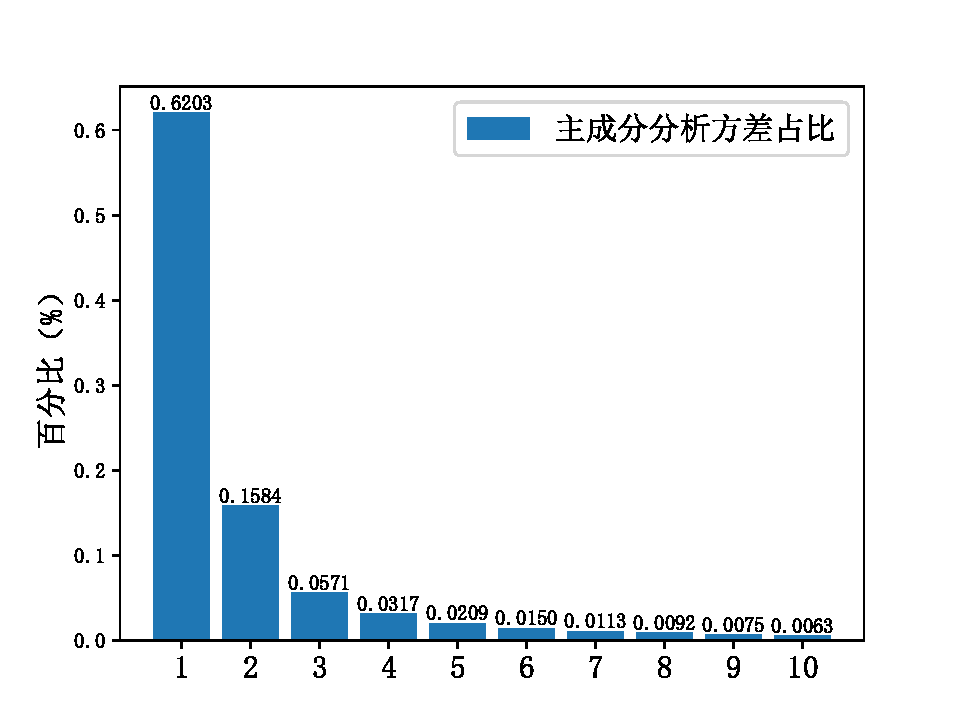
\includegraphics[width=13cm]{histogram.pdf}
    \caption[主成分分析方差占比]
      {在CIFAR-10上训练Resnet-20的前40个轮次训练轨迹在主成分分析(PCA)降维后,前10个主要维度/方向的方差占比。}
   \label{fig:dldr:pca_ratio}
  \end{figure}
  

在训练阶段中,目标子空间中低秩训练的训练集准确度变化如图\ref{fig:dldr:training}所示。从图中可以观察到,低秩降维训练情况下,模型能够相对常规随机梯度下降方法能够更快收敛。

\begin{figure}[!htp]
    \centering
    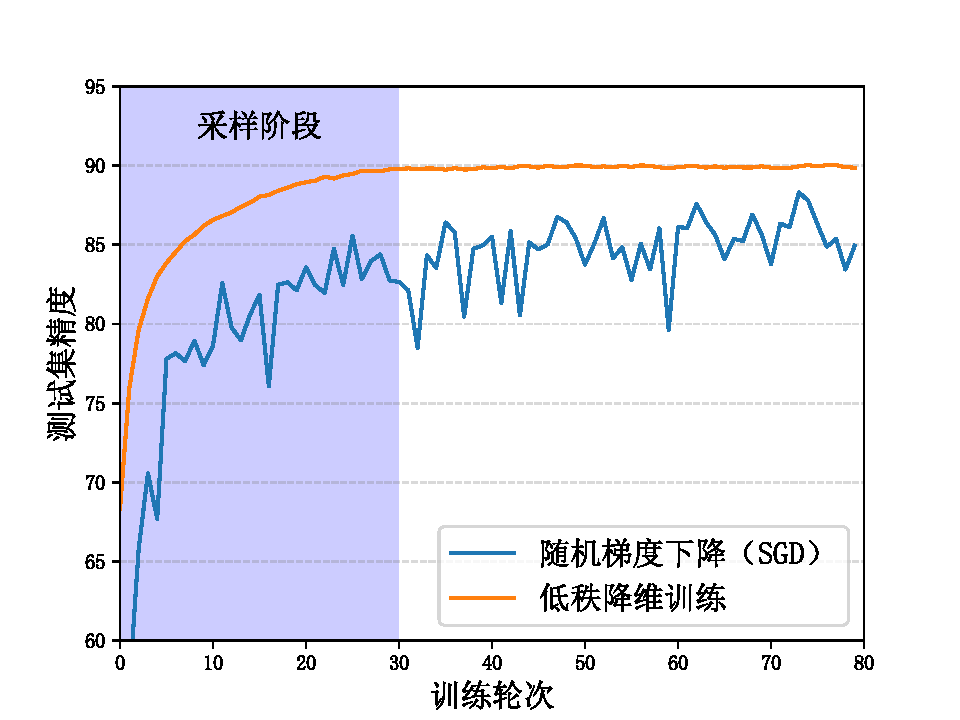
\includegraphics[width=13cm]{sgd_psgd_acc.pdf}
    \caption[中心化低秩降维实验测试集精度变化]
      {随机梯度下降(SGD)和低秩降维训练在CIFAR-10上训练Resnet-20的测试集精度变化}
   \label{fig:dldr:training}
  \end{figure}

在低秩训练的第$7$轮,模型训练集精度已达到并超过采样阶段结束时(第$40$轮)的精度,这表明低秩训练算法能够超越采样阶段结果的限制,从数据中持续学习到更多的信息以提升分类能力。

在低秩训练的第$20$轮,模型训练精度已超过常规随机梯度下降训练结束时的精度,且在后续的训练中继续收敛,最终达到$90.03\%$的精度。这表明低秩训练情况下,模型能达到乃至超过在同等超参数下的随机梯度下降训练的性能。这一性能上的优越性可能来源于低秩降维过程所带来的降噪效果(de-noising),这一点可以在未来进行深入探究。

以上结果表明,我们能够以相当低的维度在CIFAR-10上高效地训练Resnet-20,在一定程度上为低维轨迹假设\ref{hyp:low_dimensional}提供有力支持。

\section{本章小结}

在本章中,我们介绍了给本文后续研究提供主要参考的低维轨迹假设(即假设\ref{hyp:low_dimensional})。为了对该假设进行验证,本章介绍了动态线性降维方法(DLDR,即算法\ref{algo:dldr}),给出基于模型训练轨迹的低秩降维方法。根据该降维方法,本章给出了基于轨迹降维的训练算法,分为采样、降维、训练三个阶段。在验证性实验部分,本文给出了使用Resnet-20结构在CIFAR-10上按照基于轨迹降维的训练算法的实验设计,在实验结果中观察到了该训练算法下能够在低秩子空间进行训练的能力,且性能相比常规随机梯度下降方法在收敛速度、精度上有一定优势。通过本章的研究,我们能在一定的模型、数据集条件下支持低维轨迹假设,且给出一个实现的思路,为后文在联邦学习场景下进行降维压缩打下坚实的基础。




\chapter{TinyFed方法}

根据上一章所介绍并初步验证的低秩轨迹假设\ref{hyp:low_dimensional},我们给出在联邦学习场景下基于模型训练轨迹进行低秩降维压缩方法,简称为TinyFed方法(后文均简称为TinyFed)。在本章中,我们将介绍低秩轨迹假设在联邦学习框架应用的主要意义和难点,而后将给出TinyFed方法的具体算法思路及实现,并以具体数据集中的实验设计对该算法的性能进行评估,最后给出一系列消融性实验作为补充。

\section{TinyFed方法背景}

本小节中我们将结合降维压缩的相关工作给出低秩轨迹假设以及动态线性降维方法在联邦学习中应用的意义和难点。

\subsection{低秩轨迹假设在联邦学习中应用的意义}

由绪论和相关工作中的一些介绍我们知道,通信效率问题是制约联邦学习发展的一大瓶颈,在当客户端数量成百上千时,每一轮迭代中系统内所有客户端上传模型更新与下载全局模型所需的时间便愈发庞大。因此若能在低秩轨迹假设的基础上,令每一轮迭代过程中,客户端仅需上传降维压缩后的模型更新信息(相对于原本整个模型参数只需几千乃至几十的浮点数),能够极大提升联邦学习中通信效率。

在现有的降维压缩方法研究中,通常采取将神经网络模型分不同的结构进行降维,如单独对多层感知机(multi-layer perceptron)的参数矩阵进行降维或对卷积神经网络(convolutional neural network)结构进行降维。这样的策略确实能够根据网络结构特点应用常规低秩分解(如主成分分析)方法,然而也存在局限:将神经网络各个组成部分分开单独降维,忽视了各个组成部分的参数间亦存在一定的相关性,会导致降维压缩的结果仍存在一定冗余。这也是现有方法中降维目标子空间维度仍数以千计的原因(如\parencite{li2018measuring}将LENET结构降维压缩至$2900$维)。而基于轨迹的低秩降维方法,能够将模型的所有参数作为压缩的对象,在上一章的实验中能够达到在降维到$20$个独立变量的情况下进行训练,且性能接近甚至优于常规随机梯度下降方法。因此,低秩轨迹假设

\subsection{低秩轨迹假设在联邦学习中应用的难点}

\section{TinyFed方法思路及算法}

\subsection{轨迹采样阶段}

\subsection{低秩降维及降维矩阵分发阶段}

\subsection{TinyFed训练阶段}


\section{联邦学习场景下实验部分}

\subsection{数据集及划分}

\subsection{模型结构}

\subsection{实验设计}

\subsection{实验结果}


1. 利用模型训练轨迹进行模型降维压缩
在前期对比各类模型压缩方法后,本课题选择采用PCA降维的方法来降低模型通信开销。采用降维方法后的联邦学习一轮训练过程为:
1. 本地训练:所有客户端根据自身存储的数据计算梯度或参数,并根据特定的降维PCA(主成分)矩阵压缩本地模型,将压缩后的模型上传至服务端。
2. 模型聚合:服务端聚合各个客户端上传的压缩后模型,并根据特定的降维PCA矩阵的逆矩阵重建压缩后的模型。
3. 参数广播:服务端将聚合后的模型参数广播给所有的客户端
4. 模型更新:所有的客户端根据聚合的模型参数将自身的模型进行更新,并测试更新后的模型性能。

采用降维方法后,每一轮通信中,客户端与服务端的通信量将减少到降维后的参数向量大小。
在具体的降维策略上,常规的方法通常为在每一轮训练中都进行一次PCA的计算,得到降维矩阵进而进行模型压缩。本课题组在研究后认为,这一方法在每一轮中都需要进行额外的计算,且每一轮单独进行降维的效果并不能让人满意。本课题组在参考针对深度神经网络的研究论文后,决定采用基于训练轨迹的降维方法,其过程如下:
1. 采样阶段:系统按照正常联邦学习训练过程进行若干轮训练,且服务器将每一轮聚合后得到的模型保存下来(即保存训练轨迹)。
2. 计算降维矩阵:服务器将前若干轮的模型组接成一个大矩阵,利用PCA方法计算得到降维矩阵,并将此矩阵分发给各个客户端。
3. 本地训练及上传:每个客户端在后续的训练中根据分发的降维矩阵,按照前述方法对本地模型进行降维并上传。
4. 云端聚合:服务端获得各个客户端上传的压缩后的模型,也利用2中得到的PCA矩阵从压缩后的模型中重建原本的模型。
5. 重复进行3和4,直至模型收敛

\chapter{在基于轨迹降维的联邦学习框架中应用差分隐私}
\input{contents/math_and_citations}
\input{contents/floats}
\input{contents/summary}

%TC:ignore

% 参考文献
\printbibliography[heading=bibintoc]

% 附录
\appendix

% 附录中图表不加入索引
\captionsetup{list=no}

% 附录内容
\input{contents/app_maxwell_equations}
\input{contents/app_flow_chart}

% 结尾部分
\backmatter

% 用于盲审的论文需隐去致谢、发表论文、科研成果、简历

% 致谢
\input{contents/acknowledgements}

% 发表论文及科研成果
% 盲审论文中,发表论文及科研成果等仅以第几作者注明即可,不要出现作者或他人姓名
\input{contents/achievements}

% 简历
\input{contents/resume}

% 学士学位论文要求在最后有一个大摘要,单独编页码
\input{contents/digest}

%TC:endignore

\end{document}
